\documentclass{beamer}

\usepackage[UTF8,noindent]{ctexcap}
\usepackage{color}%引入颜色
\usetheme{Berlin}%使用Singapore主题
\usepackage{graphicx}%引入插图
\usepackage{ulem}%删除线
\usepackage{tikz}
\usefonttheme[onlymath]{serif}
\usepackage{minted}%[fragile]
\useoutertheme{infolines}
%\usepackage[orientation=landscape,size=custom,width=16,height=9,scale=0.5,debug]{beamerposter}

\title{OI 代数选讲}
\date{2021年7月17日}
\author{租酥雨}
\begin{document}\small
	
%\usebackgroundtemplate{\tikz\node[inner sep=0pt,opacity=0.3]{\includegraphics[width=16cm,height=9cm]{zsy_background.jpg}};}
	\begin{frame}
	\titlepage
		\begin{center}
		%
\includegraphics[width=2.0cm]{cj.jpg}
		
\includegraphics[width=2.0cm]{zsy.jpg}
		\end{center}
	\end{frame}
\section{outline}
\begin{frame}{outline}
	\begin{itemize}
		\item 代数结构
		\item 模$p$整数环(同余)
		\item 质数分解
		\item 积性函数与筛法
		\item 离散对数
		\item 线性代数选讲
	\end{itemize}
\end{frame}

\section{代数结构}
\begin{frame}{群(Group)}
	对于非空集合$G$以及$G$上的二元运算$\circ: G \times G \to G$,若满足:
	\begin{itemize}
		\item 结合律,即$\forall x, y, z \in G, (x \circ y) \circ z = x \circ (y \circ z)$;
		\item 单位元存在,即存在$e \in G$使得$\forall x \in G, e \circ x = x \circ e = x$;
		\item 逆元存在,即$\forall x \in G, \exists y \in G, x \circ y = y \circ x = e$,此时$y$称为$x$的逆元,记为$x^{-1}$。
	\end{itemize}
	
	则称$(G, \circ)$构成一个群(Group)。(有时也会说$G$关于$\circ$构成一个群)\\
	
	若群$(G, \circ)$还对$\circ$满足交换律,则称之为交换群或阿贝尔群。\\
	
	e.g. 所有$n$元置换关于置换的复合运算构成一个群(不是阿贝尔群)。
\end{frame}
\begin{frame}{环(Ring)}
	对于非空集合$R$以及$R$上的两种运算$\oplus, \otimes: R \times R \to R$,若满足:
	\begin{itemize}
		\item $R$关于$\oplus$构成一个阿贝尔群;(特别的,我们接下来将群$(R, \oplus)$中的\textbf{单位元,逆元}称作\textbf{零元、负元})
		\item $R$对$\otimes$有结合律,即$\forall x, y, z \in R, (x \otimes y) \otimes z = x \otimes (y \otimes z)$;
		\item 对$\oplus, \otimes$有左右分配率,即$\forall x, y, z \in R$,有\begin{align*}x \otimes(y \oplus z) = x \otimes y \oplus x \otimes z\\(x \oplus y) \otimes z = x \otimes z \oplus y \otimes z
		\end{align*}
	\end{itemize}
	
	则称$(R, \oplus, \otimes)$构成一个环(Ring)。\\
	
	e.g. 多项式关于多项式加法与乘法构成一个环(是一个有$1$的交换环);所有$n$阶矩阵关于矩阵的加法与乘法构成一个环(有单位元$E = \mathrm{diag}\{1, 1, \cdots, 1\}$)。
\end{frame}

\begin{frame}{域(Field)}
	对于非空集合$F$以及定义在$F$上的两种运算$\oplus, \otimes: F \times F \to F$,若满足:
	\begin{itemize}
		\item $(F, \oplus, \otimes)$是一个环;
		\item $F$对$\otimes$有交换律;
		\item 单位元存在,即存在$e \in F$使得$\forall x \in F, e \circ x = x \circ e = x$;
		\item 逆元存在,即$\forall x \in F$且$x \neq 0$, $\exists y \in G, x \circ y = y \circ x = e$,此时$y$称为$x$的逆元,记为$x^{-1}$。
	\end{itemize}

	则称$(F, \oplus, \otimes)$构成一个域(Field)。\\
	
	前面提及的“有$1$的交换环”,其实指的是多项式环只是不满足“逆元存在”这条域的性质。
\end{frame}
\begin{frame}{一些性质}
	上述代数结构中提及的单位元、逆元,都是唯一的。\\\pause
	
	域中不存在非平凡零因子。($\forall x, y \in F, xy = 0 \Rightarrow x = 0 $或$ y = 0$)\\\pause
	
	最小的数域是有理数域$\mathbb Q$。(Q:包含$\sqrt 2 / \sqrt[n]{2} / \mathrm i / \omega_n$的最小数域是什么?)\\\pause
	
	模$p$整数环$\mathbb Z_p$是一个域当且仅当$p$是质数。(必要?充分?)\\
	\pause
	
	总结一下就是:群只有一种运算;域是优美的,环不够优美。
	
\end{frame}
	\section{模$p$整数环(同余)}
\begin{frame}{欧几里得算法及其扩展}
	求$\gcd(a,b)$?
	\pause\\
	
	求$ax+by=\gcd(a,b)$的一组整数解?
	\pause\\
	
	由$\gcd(a,b)=\gcd(b,a \bmod b)$可得:
	
	$$ax_1+by_1=bx_2+(a-\lfloor\frac{a}{b}\rfloor b)y_2$$
	
	该不定方程的一组特解为:
	
	$$\begin{cases}
		x_1=y_2\\
		y_1=x_2-\lfloor\frac{a}{b}\rfloor y_2
	\end{cases}$$
	
	递归到$b=0$时存在一组特解$\begin{cases}x=1\\y=0\end{cases}$。
\end{frame}
\begin{frame}{线性求逆元}
	在$O(n)$时间内求出$1...n$在模$p$意义下的逆元。
	
	$$\begin{aligned}
		i\times \lfloor\frac{p}{i}\rfloor + (p \bmod i) &\equiv 0 &\mod p\\
		i\times \lfloor\frac{p}{i}\rfloor &\equiv -(p \bmod i) &\mod p\\
		i^{-1} &\equiv -\lfloor\frac{p}{i}\rfloor \times (p \bmod i)^{-1} &\mod p 
	\end{aligned}$$
	
	这种求法同样适用于$p$不为质数的情况。
	\\
	
	当然也可以使用$O(n+\log p)$的方法(不限值域),但要注意去除与$p$不互质(不存在逆元)的数。
\end{frame}
\begin{frame}{中国剩余定理}
	假设$p_1,p_2,...,p_k$两两互质,并记$P=\prod\limits_{i=1}^kp_i$,则同余方程组
	
	$$\begin{cases}
		x \equiv a_1 \mod p_1\\
		x \equiv a_2 \mod p_2\\
		...\\
		x \equiv a_k \mod p_k
	\end{cases}$$
	
	的最小整数解为$\sum\limits_{i=1}^ke_iw_ia_i \mod P$,其中$w_i=\frac{P}{p_i}, e_iw_i \equiv 1 \mod p_i$。
\end{frame}
\begin{frame}{费马小定理}
	若$p$为质数,则$a^{p-1} \equiv 1 \mod p$。
	\\
	
	注意到对于$\mathbb Z_p$中非零元$a$,下述映射\begin{align*}
		\sigma_a: \mathbb Z_p &\to \mathbb Z_p\\
		x &\mapsto ax
		\end{align*}
	是双射,从而有$\prod\limits_{x \in \mathbb Z_p, x \neq 0}x = \prod\limits_{x \in \mathbb Z_p, x \neq 0}ax$,两边同消去$x^{p-1}$得到结论。\\
	
	常使用$a^{p-2}\equiv a^{-1} \mod p$来求逆元。
\end{frame}
\begin{frame}{欧拉定理及其扩展}
	若$\gcd(a, n) = 1$,则$a^{\varphi(n)} \equiv 1 \mod n$。
	\\
	
	记$U(\mathbb Z_n)$表示$\mathbb Z_n$中的可逆元集合,证明方式与费马小类似,构造一个$U(\mathbb Z_n)$到$U(\mathbb Z_n)$的双射即可。\\
	
	可以发现费马小定理是欧拉定理在$n$为质数时的推论。
	\\
	
	若$\gcd(a,n)\neq 1$,则
	
	$$a^b\equiv\begin{cases}
		a^b &b < \varphi(n)\\
		a^{b \bmod \varphi(n)+\varphi(n)} &b \ge \varphi(n)
	\end{cases}
	\mod n$$
	
\end{frame}

\section{质数分解}
\begin{frame}{唯一分解定理}
	任意正整数都可以被唯一分解成若干质数的乘积。
	
	$$n = \prod_{i=1}^k p_i^{\alpha_i}$$
	
	接下来可能会不加说明地使用如上定义。
		
	\begin{center}
		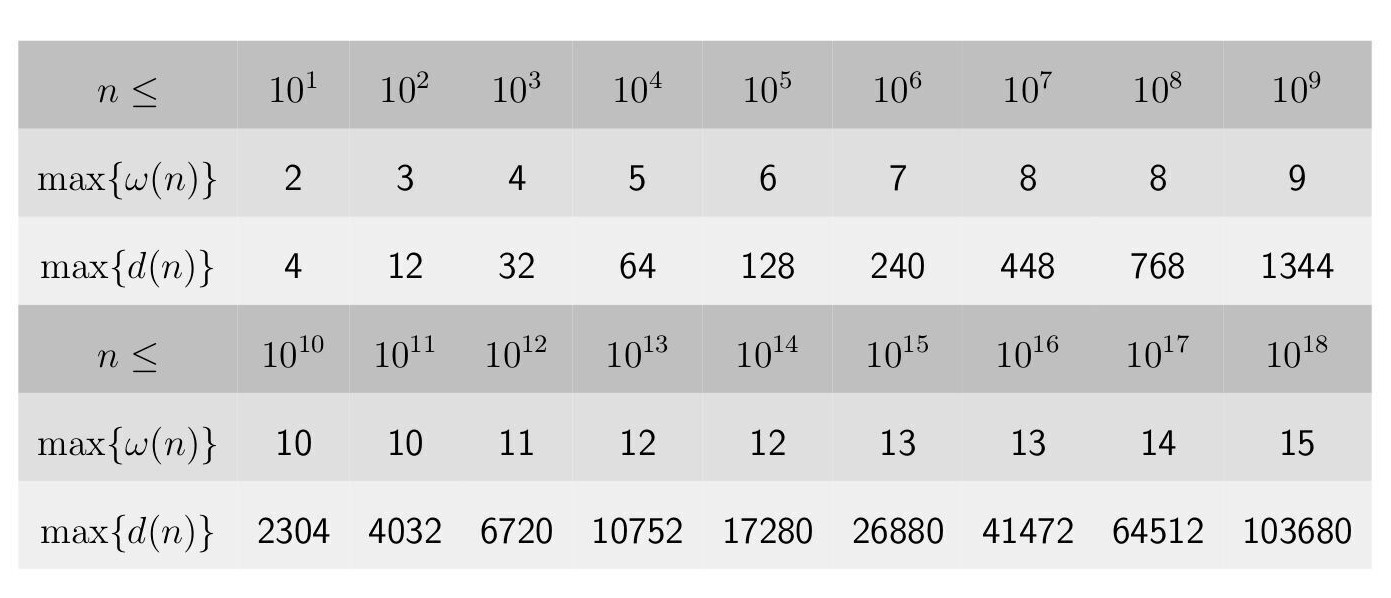
\includegraphics[width=9.0cm]{biao.jpg}
	\end{center}

	这里$\omega(n), d(n)$分别表示$n$不同质因子个数以及约数个数。
\end{frame}
\begin{frame}{质数分解算法}
	\begin{block}{$O(\sqrt n)$分解}
		由于$n$只包含至多$1$个大于$\sqrt n$的质因子,所以可以枚举所有小于等于$\sqrt n$的质因子试除,如果剩下的数不是$1$那就也是$n$的一个质因子。
	\end{block}
	\begin{block}{$O(n)-O(\log n)$分解}
		考虑到质因子个数是$O(\log n)$级别的,因此先$O(n)$预处理$1...n$所有数的最小质因子$d_i$,每次分解时通过不断地$x \to \frac{x}{d_x}$即可实现单次$O(\log n)$分解。
	\end{block}
	\begin{block}{Pollard's Rho 分解算法}
		是一个复杂度为$O(n^{\frac14})$的分解算法,具有比较高的实用性(比如说可以快速分解\texttt{long long}范围内的大整数)。
	\end{block}
\end{frame}
\begin{frame}{质数分解算法:Pollard's Rho 算法}
	
	质数分解等价于对于给出的非质数$n$找到它的一个非平凡因子$1 < p \le \sqrt n$,此外还需要通过 Miller-Rabin 质数测试来判断$n$是不是质数以终止递归。\\
	
	具体做法是构造一个函数$f: \mathbb Z_n \to \mathbb Z_n$使其在$\bmod p$下几乎是随机的,且$f(x) \equiv f(x + p) \bmod p$。在$\bmod p$下,从一个固定点$x_0$出发的$x \to f(x)$呈现出$\rho$型结构,而我们一旦找到了两个数$f^{(a)}(x_0) \equiv f^{(b)}(x_0) \bmod p$,由于两者在$\bmod n$下大概率不相等,我们便可以得到$p$的某个倍数,与$n$取$\gcd$便可以得到$n$的一个非平凡因子。\\
	
	实现中一般取$f(x) = x^2 + c$,同时需要注意的一个问题是$\rho$型结构的期望大小,这个问题等价于期望选多少个数能存在两个模$p$相同的,根据生日悖论,大约是$\sqrt p$的规模。\\
	
	由于$n$除去最大因子后的约数和是$O(\sqrt n)$,因此总复杂度大概是$O(n^{\frac14}\log n)$,$\log n$源于求$\gcd$,实际上是可以多次合并在一起判的。
	
\end{frame}

\section{积性函数与筛法}
\begin{frame}{积性函数}
	数论函数大概就是指把正整数映到其他什么数域上去的函数。
	\\
	
	若$f(n)$为数论函数,$f(1)=1$,且对于任意互质的正整数$p,q$均满足$f(pq) = f(p)f(q)$,则称$f(n)$为积性函数。
	\\
	
	若$f(n)$为积性函数,且对于任意正整数$p,q$均满足$f(pq) = f(p)f(q)$,则称$f(n)$为完全积性函数。
\end{frame}
\begin{frame}{常见积性函数}
	莫比乌斯函数$\mu(n)=\prod\limits_{i=1}^k-[\alpha_i=1]$
	\\
	
	欧拉函数$\varphi(n)=\sum\limits_{i=1}^n[\gcd(i,n)=1]=\prod\limits_{i=1}^k(p_i-1)p_i^{\alpha_i-1}$
	\\
	
	除数函数$\sigma_x(n)=\sum\limits_{d|n}d^x=\prod\limits_{i=1}^k\sum\limits_{j=0}^{\alpha_i}p_i^{xj}=\prod\limits_{i=1}^k\frac{1-p_i^{x(\alpha_i+1)}}{1-p_i^x}$
	\\
	
	单位元函数$e(n)=[n=1]$
	\\
	
	恒等函数$I(n)=1$
	\\
	
	幂函数$id_x(n)=n^x$
\end{frame}
\begin{frame}{Dirichlet 卷积}
	数论函数$f(n)$与$g(n)$的 Dirichlet 卷积为$(f*g)(n)=\sum\limits_{d|n}f(d)g(\frac nd)$,当$f$和$g$均为积性函数时,$f * g$也是积性函数。
	\\
	
	积性函数关于 Dirichlet 卷积构成一个有单位元$e(n) = [n = 1]$的交换环,其中的可逆元是所有满足$f(1) \neq 0$的函数。

\end{frame}
\begin{frame}{常见 Dirichlet 卷积}
	\pause
	大家都知道
	
	$$\sum_{d|n}\mu(d)=[n=1],\sum_{d|n}\varphi(d)=n$$
	\pause
	
	写成Dirichlet卷积的形式就是
	
	$$\mu * I = e, \varphi * I = id_1$$
	\pause
	
	那么就很显然可以看出
	
	$$\mu * id_1 = \varphi$$
	\pause
	
	也即
	
	$$\sum_{d|n}d\mu(\frac{n}{d})=\varphi(n)$$
\end{frame}
\begin{frame}{筛法}
	\begin{block}{埃氏筛法}
		枚举每个质数并筛去其倍数,时间复杂度$O(n\log\log n)$。
	\end{block}
	\begin{block}{欧拉筛法(线性筛)}
		枚举每个数$n$,从小到大枚举质数$p \le p_1$并把$n\times p$筛掉,这样可以保证所有数只会被其最小质因子筛掉一次。
	\end{block}
\end{frame}
\begin{frame}{杜教筛}
	假设要求前缀和的积性函数为$f(n)$,记之前缀和为$S(n)=\sum\limits_{i=1}^nf(i)$。
	
	构造 Dirichlet 卷积$h = f * g$。
	
	$$
	\begin{aligned}
		h(i)&=\sum_{d|i}f(\frac{i}{d})g(d)\\
		\sum_{i=1}^nh(i)&=\sum_{i=1}^n\sum_{d|i}f(\frac{i}{d})g(d)\\
		&=\sum_{d=1}^ng(d)\sum_{d|i}^nf(\frac{i}{d})\\
		&=\sum_{d=1}^ng(d)S(\lfloor\frac{n}{d}\rfloor)
	\end{aligned}
	$$
	
	于是有$g(1)S(n)=\sum\limits_{i=1}^nh(i)-\sum\limits_{d=2}^ng(d)S(\lfloor\frac{n}{d}\rfloor)$。一般会把$g, h$构造地比较简单,然后直接递归求所有$S(\frac{n}{d})$。
\end{frame}
\begin{frame}{杜教筛的时间复杂度证明}
	可以发现在求$S(n)$的过程中,只会递归调用到$S(\lfloor\frac{n}{d}\rfloor)$,同时还需要$O(\sqrt n)$的复杂度进行累加(这里认为$g$和$h$均可以在$O(1)$的时间内求任意前缀和),因此若实现记忆化,时间复杂度大约是
	
	$$\sum_{x=1}^{\sqrt n}O\left(\sqrt x\right)+O\left(\sqrt \frac nx\right)$$
	
	积分可知时间复杂度为$O(n^{\frac 34})$。
	
	考虑加以预处理,假设预处理出前$k$项的前缀和,则时间复杂度为
	
	$$O(k)+\sum_{x=1}^{\frac nk}O\left(\sqrt \frac nx\right)$$
	
	积分可知时间复杂度为$O\left(k+\frac{n}{\sqrt k}\right)$,当$k$取$O(n^{\frac 23})$时取到最优时间复杂度$O(n^{\frac 23})$。
\end{frame}
\begin{frame}{(若干年前的)Min\_25筛}
	筛法的过程大致分为两步:先对所有$x=\lfloor\frac nd\rfloor$筛出不超过$x$的所有质数的$f$值之和,再求出剩下的合数的$f$值之和。定义$g(i)$为所有数按照$f(i)$在$i$为质数时的式子算出来的结果,并记$pri_j$表示第$j$小的质数。
	
	设$G(i,j)$表示$i$以内所有质数以及最小质因子$>pri_j$的合数的$g$之和。从小到大枚举质因子$p$,把最小质因子恰为$pri_j$的合数去掉,这要求能在已知$\sum g(i)$的前提下快速计算$\sum g(i\times pri_j)$。枚举$\ge pri_j^2$的所有$i$,$G(i,j)$需要去掉的部分是$G(\lfloor \frac{i}{pri_j} \rfloor,j-1)-sum_{j-1}$并把每个数从$g(i)$变成$g(i\times pri_j)$,其中$sum_j$表示前$j$个质数的$f$值之和。
	
	接下来就用所有质数的$f$来求出剩下的合数的$f$。设$F(i,j)$表示$i$以内所有质数以及最小质因子$>pri_j$的合数的$f$之和。从大到小枚举质因子$pri_j$,枚举$\ge pri_j^2$的所有$i$,再枚举一个$pri_j^{k+1}\le i$的$k$,把$F(\lfloor\frac {i}{pri_j^k}\rfloor,j) \times f(pri_j^k) + f(pri_j^{k+1})$累加进$F(i,j-1)$。
	
	最终可以实现对所有$x=\lfloor\frac nd\rfloor$筛出不超过$x$的$f$值之和。
	
\end{frame}
\begin{frame}{Min\_25 筛的时间复杂度证明}
	
	对于一个数$x$,满足$p^2 \le x$的质数$p$的个数是$O(\frac{\sqrt x}{\log \sqrt x})$级别的。
	
	只考虑Min\_25筛中前一部分的时间复杂度。类似杜教筛,由于只需要求所有$\lfloor\frac{n}{d}\rfloor$处的前缀和,总时间复杂度是
	
	$$\sum_{x=1}^{\sqrt n}O\left(\frac{\sqrt x}{\log \sqrt x}\right)+O\left(\frac{\sqrt{\frac nx}}{\log \sqrt{\frac nx}}\right)$$
	
	所有的$\log$都是同级的,提出后复杂度就和不加预处理的杜教筛完全一样,因此时间复杂度为$O\left(\frac{n^{\frac 34}}{\log n}\right)$。
	
	后一部分需要额外枚举质数$p$的出现次数$k$,复杂度(大概/也许/可能)不会差太多。
	
\end{frame}

\begin{frame}{关于推式子}
	一般可以利用两个重要结论$$n = \sum_{d | n}\varphi(d), [n = 1] = \sum_{d | n}\mu(d)$$
	
	以及数论分块的技巧:$\lfloor\frac{n}{d}\rfloor$只有$O(\sqrt n)$种取值。
	
	更多的技巧就靠大家在实践中体会吧(因为我已经不太记得了)
\end{frame}

\begin{frame}{bzoj2154 Crash的数字表格}
	\begin{block}{description}
		给出$n, m$,求$$\sum_{i=1}^n\sum_{j=1}^m\mathrm{lcm}(i,j)$$
	\end{block}
	\begin{block}{constraint}
		$1 \le n, m, \le 10^7$
	\end{block}
\end{frame}
\begin{frame}{bzoj2154 Crash的数字表格 solution}
		\begin{align*}
		ans &= \sum_{i=1}^n\sum_{j=1}^m\frac{ij}{\gcd(i,j)}\\
		&= \sum_{d=1}^{n}\frac{1}{d}\sum_{i=1}^n\sum_{j=1}^mij[\gcd(i,j)=d]\\
		&= \sum_{d=1}^{n}d\sum_{i=1}^{n/d}\sum_{j=1}^{m/d}ij[\gcd(i,j)=1]\\
		&= \sum_{d=1}^{n}d\sum_{i=1}^{n/d}\sum_{j=1}^{m/d}ij\sum_{x|i, x|j}\mu(x)\\
		&= \sum_{d=1}^{n}d\sum_{x=1}^{n/d}\mu(x)x^2\frac {\lfloor\frac n{xd}\rfloor(\lfloor\frac n{xd}\rfloor+1)}{2} \frac {\lfloor\frac m{xd}\rfloor(\lfloor\frac m{xd}\rfloor+1)}{2}
		\end{align*}
	做两次数论分块即可。
\end{frame}
\section{离散对数}
\begin{frame}{原根}
	假设$g$是质数$p$的一个原根,则$g^0,g^1,...,g^{p-2}$在模$p$意义下两两不同。
	\\
	
	也即,对于$\forall x\in[1,p-1]$,均存在$k\in[0,p-2]$使$x \equiv g^k \mod p$。
	\\
	
	由这种方式可以把模意义下的乘法转化成原根指数上的加法,也就是实现了模意义下的离散对数。
	
\end{frame}
\begin{frame}{大步小步算法}
	给出$a,b,p$,求$x$使$a^x \equiv b \mod p$。
	\pause\\
	
	分块,令$k=\lceil\sqrt p\rceil$,设$x=ky-z$,则有$a^{ky}=b\times a^z$。
	
	显然$y,z \in [0,k]$,因此预处理出所有$a^{ky}$并哈希存储,再枚举$z$判断是否存在相等的即可。
	\pause\\
	
	这个做法要求$\gcd(a,p)=1$,因为推导过程中用到了$a$在模$p$意义下的逆元。
\end{frame}

\begin{frame}{二次剩余、Cipolla 算法}
	
	对于同余方程$x^2 \equiv n \mod p$,判断是否有解,有解的话求解。这次我们只在$p$为奇素数的情况下讨论这个问题,首先排除$n=0$这种平凡的情况。\\
	
	不加证明地给出一些关于二次剩余的性质:
	
	\begin{itemize}
		\item $x^2 \equiv n \mod p$若有解则恰好有两个解;
		\item $[1, p)$中恰好有一半的$n$对上面那个方程有解;
		\item $n^{\frac{p-1}{2}} \equiv 1 \Leftrightarrow $方程有解,$n^{\frac{p-1}{2}} \equiv -1 \Leftrightarrow $方程无解。
	\end{itemize}
	
	Cipolla算法可以对有解的同余方程$x^2\equiv n \mod p$求解,做法是先找出一个$a$使得$a^2 - n$没有二次剩余,定义$\omega = \sqrt{a^2-n}$(需要扩域),那么$(a + \omega)^p = a^p + \omega^p = a - \omega, (a + \omega)^{p+1} = a^2-\omega^2 = n$,于是只要求出$(a+\omega)^{\frac{p+1}{2}}$就行了。(需要证明一下$(a+\omega)^{\frac{p+1}{2}} \in \mathbb Z_p$)
	
\end{frame}
\section{例题}
\begin{frame}{apio2019 奇怪装置}
	\begin{block}{description}
		有一个奇怪的装置,在$t$时刻会显示数对$((t+\lfloor\frac tB\rfloor) \bmod A, t \bmod B)$。给出$n$个不交的连续时间段$[l_i,r_i]$,问这个装置在这些时间段内会显示出多少种不同的数对。
	\end{block}
	\begin{block}{constraint}
		$1 \le n \le 10^6, 1 \le A, B \le 10^{18}, 0 \le l_i \le r_i \le 10^{18}.$
	\end{block}
	\pause
	\begin{block}{solution}
		可以发现存在循环节$\frac{AB}{\gcd(A,B+1)}$。
		
		因此所有区间对循环节取模,问题变成在$[0,\frac{AB}{\gcd(A,B+1)})$上的覆盖问题,差分统计即可。
	\end{block}
\end{frame}
\begin{frame}{snoi2019 数论}
	\begin{block}{description}
		给出正整数$P,Q,T$,大小为$n$的整数集$A$和大小为$m$的整数集$B$,求:
		
		$$\sum_{i=0}^{T-1}[i \bmod P \in A][i \bmod Q \in B]$$
		
		换言之,就是求有多少小于$T$的非负整数$x$满足$x$除以$P$的余数属于$A$且$x$除以$Q$的余数属于$B$。
	\end{block}
	\begin{block}{constraint}
		$1 \le n, m, P, Q \le 10^6, 1 \le T \le 10^{18}.$
	\end{block}
	\pause
	\begin{block}{solution}
		$x\to (x+P) \bmod Q$会形成$\gcd(P,Q)$个长度为$\frac{Q}{\gcd(P,Q)}$的环。
		
		枚举$x\bmod P$的值(即枚举$a_i$),问题变成求有多少$0\le x\le \lfloor\frac{T-1-a_i}{P}\rfloor$满足$(Px+a_i)\bmod Q\in B$。其实就是求从$a_i$出发走$\lfloor\frac{T-1-a_i}{P}\rfloor$步能到达的所有点的点权和。根据环长讨论一下即可,复杂度$O(P+Q)$。
	\end{block}
\end{frame}
	\begin{frame}{51nod1769 Clarke and math 2}
	\begin{block}{description}
		已知数论函数$f(n),g(n)$满足
		
		$$g(i)=\sum_{i_1|i}\sum_{i_2|i_1}...\sum_{i_k|i_{k-1}}f(i_k)$$
		
		给出$f(1)...f(n)$,求$g(1)...g(n)$对$10^9+7$取模后的结果。
	\end{block}
	\begin{block}{constriction}
		$1 \le n \le 10^5, 1 \le k \le 10^{10^5}, 0 \le f(i) < 10^9+7.$
	\end{block}
	\pause
	\begin{block}{solution}
		写成Dirichlet卷积的形式是$g=f*I^k$。
		
		考虑$I^k(n)$怎么求。这是一个积性函数,因此只需要考虑$I^k(p^{\alpha})$怎么求即可。这等价于长度为$k$值域为$[0,\alpha]$的单调不降序列方案数,等价于把$\alpha$个球放入$k$个盒子里的方案数,即$\binom{\alpha+k-1}{\alpha}$。
	\end{block}
\end{frame}

\begin{frame}{codeforces1097D Makoto and a Blackboard}
	\begin{block}{description}
		有一个数$n$,每次操作为随机选择$n$的一个约数$m$并将$n$替换成$m$,求$k$次操作后$n$的期望值模$10^9+7$。
	\end{block}
	\begin{block}{constraint}
		$1 \le n \le 10^{15}, 1 \le k \le 10^4.$
	\end{block}
	\pause
	\begin{block}{solution}
		根据乘法分配律,只需要对每个$p_i^{\alpha_i}$求出答案即可。
		
		只需要考虑指数。问题转化成给一个数$\alpha_i$,每次把当前的数$x$等概率随机变成$[0,x]$的一个整数,求$k$次操作后剩下的数是$[0,\alpha_i]$的概率。
		
		直接$O(\alpha_i^2k)$暴力dp或者$O(\alpha_i^3\log k)$矩乘。
	\end{block}
\end{frame}
\begin{frame}{codeforces1097F Alex and a TV Show}
	\begin{block}{description}
		你需要编写一种数据结构来维护$n$个可重集合,支持四种操作:
		\begin{itemize}
			\item 将$S_x$设为$\{v\}$
			\item 将$S_x$设为$S_y + S_z$,操作后$|S_x|=|S_y|+|S_z|$
			\item 将$S_x$设为$S_y\times S_z$,这里的$A \times B$定义为$\{\gcd(a,b)|a\in A, b\in B\}$,操作后$|S_x|=|S_y|\times|S_z|$
			\item 询问$S_x$中$v$元素的数量
		\end{itemize}
		
		由于一些原因,你只需要输出每个询问的答案对$2$取模后的结果。
	\end{block}
	\begin{block}{constraint}
		$1\le n, m \le 10^5, 1 \le v \le 7000.$
	\end{block}
\end{frame}
\begin{frame}{codeforces1097F Alex and a TV Show}
	\begin{block}{solution}
		对每个可重集维护一个数组$a_i$表示可重集中有多少个数是$i$的约数,可以发现这样的$a$数组可以唯一的表示一个可重集。
		
		第二种操作本质是$a$数组对应位相加,第三种操作本质是$a$数组对应位相乘,这个结论读者自证不难。
		
		由于只需要输出$\bmod 2$意义下的答案,所以可以用一个\texttt{bitset<7000>}来维护$a$数组,这样对应位相加变成了按位异或,对应位相乘变成了按位与。
		
		维护$a$数组后,对于一次询问$v$,答案为$\sum_{v|u}a_u\mu(\frac{u}{v})$,由于$-1 \equiv 1 \bmod 2$,所以只需要再维护$7000$个\texttt{bitset<7000>}表示询问$v$时哪些位的莫比乌斯函数不为零就好了。
		
		时间复杂度为$O(\frac{7000m}{\omega})$。
	\end{block}
\end{frame}



\section{线性代数选讲}
\begin{frame}
\begin{center}
	{\Huge 线性代数选讲}
\end{center}
\end{frame}

\begin{frame}[fragile]{线性方程组}
	说到解线性方程组大家应该都会高斯消元,其大致流程就是\sout{做消消乐}用一行中的$x_i$把其他行中的$x_i$都消掉,最后系数会长成上三角的形式。
	
	下面展示了一份保证有\textbf{唯一解}时的高斯消元板子,数组\texttt{a}前$n$列存的是方程组的系数,第$n + 1$列存的是方程等式右侧的值。
\begin{minted}{c++}
for(int i = 1; i <= n; ++i){
    if(a[i][i] == 0){
        for(int j = i + 1; j <= n; ++j)
            if(a[j][i] != 0){
                swap(a[i], a[j]);
                break;
            }
    }
    for(int j = i + 1; j <= n; ++j){
        double t = a[j][i] / a[i][i];
        for(int k = i; k <= n + 1; ++k)
            a[j][k] -= a[i][k] * t;
    }
}
\end{minted}
\end{frame}

\begin{frame}{线性方程组的解:唯一解/多解/无解?}
	但是高斯消元怎么处理多解或者是无解的情况呢?\\
	
	从代数的角度思考,对于给定的线性方程组$$\begin{cases}
		a_{11}x_1 + a_{12}x_2 + \cdots + a_{1n}x_n = b_1\\
		a_{21}x_1 + a_{22}x_2 + \cdots + a_{2n}x_n = b_2\\
		\vdots\\
		a_{m1}x_1 + a_{m2}x_2 + \cdots + a_{mn}x_n = b_m	\end{cases}$$
	,它有唯一解/多解/无解的等价条件分别是什么?\\
	
\end{frame}

\begin{frame}{齐次线性方程组}
	先考虑一个简单的情况:$b_i = 0, i = 1, 2, \cdots, m$,此时方程组不会无解,因为一定存在一组解$x_1 = x_2 = \cdots = x_n = 0$。\\
	
	如果在消元的过程中出现了某一行前$i-1$个系数均为零而第$i$个系数不为零,我们便称$x_i$为一个\textbf{主元}。非主元的变量称为\textbf{自由元}。\\
	
	在前面展示的代码中,如果出现了\texttt{a[i][i] == 0}的情况,就说明$x_i$是一个自由元。\\
	
	自由元顾名思义,是可以任取的,而主元依赖于自由元的取值。我们称一个系数矩阵是\textbf{简化行阶梯型矩阵},若:
	\begin{itemize}
		\item 它是阶梯型矩阵,即它是上三角的,且从上往下每行包含的主元下标递增
		\item 每个主元前的系数都是$1$
		\item 每个主元所在列其余元素都是$0$
	\end{itemize}

	\textbf{结论. }齐次线性方程组有唯一解(仅有零解)当且仅当没有自由元。
\end{frame}

\begin{frame}{非齐次线性方程组}
	现在把$b_1, b_2, \cdots, b_m$加回来,变成了一个非齐次线性方程组。对于一个非齐次线性方程组,我们把抹去常数项后得到的齐次线性方程组称为其导出组。\\
	
	\textbf{结论. }非齐次线性方程组的任意两解之差是其导出组的解。\\
	
	因此非齐次线性方程组的解唯一(没有指明存在性)当且仅当其导出组解唯一(仅有零解)。\\
	
	然后讨论一下解的存在性,只需要保证这些方程的限制能够被同时满足就行了。在这里我们不加证明地给出结论:存在解当且仅当无法通过消元得到这样的方程,其等号左边的未知量系数均为零,而右边常数项非零。
	
\end{frame}

\begin{frame}{矩阵}
	讲一下大家应该比较熟悉的矩阵。一个$n \times m$的矩阵都是把$n \times m$个数写成一个长方形,然后用圆括号框起来。$$\begin{pmatrix}
		a_{11} & a_{12} & \cdots & a_{1n}\\
		a_{21} & a_{22} & \cdots & a_{2n}\\
		\vdots & \vdots & \ddots & \vdots\\
		a_{n1} & a_{n2} & \cdots & a_{nn}
		\end{pmatrix}$$
	
	矩阵的乘法要求左边矩阵的列数等于右边矩阵的行数。一个$n \times m$的矩阵$A$乘上一个$m \times r$的矩阵$B$,会得到一个$n \times r$的矩阵$C$,其中$$C_{ij} = \sum_{k=1}^mA_{ik}B_{kj}$$矩阵乘法\textbf{不满足交换律}。\\
	
	有时我们会把一个$1 \times n$的矩阵称作行向量,把一个$n \times 1$的矩阵称为列向量。记$M_{n \times m}(K)$为定义在数域$K$上的$n \times m$矩阵集合。
\end{frame}

\begin{frame}{线性空间}
	记$K$是一个数域($\mathbb R, \mathbb C, \mathbb Q, \mathbb Z_{10^9+7}$),令$$K^n \triangleq \{(a_1, a_2, \cdots, a_n) | a_i \in K\}$$
	(就是$K$上的有序$n$元组构成的集合)并在$K^n$中自然地定义加法与数乘。一般用小写希腊字母$\alpha, \beta, \gamma, \cdots$来表示$K^n$中元素(称作\textbf{向量})。\\
	
	于是我们就可以这样地描述一个线性方程组:$$x_1\alpha_ 1+ x_2\alpha_2 + \cdots + x_n\alpha_n = \beta$$其中$\alpha_i, \beta \in K^m, x_i \in K$。\\
	
	一个$K$上的\textbf{线性空间}需要满足八条看上去比较朴素的性质(请善用搜索),而$K^n$显然是满足的。也存在其他满足性质的集合,比如说$M_{n\times m}(K)$。\\
	
	所有$K$上的线性空间都\textbf{同构}于某个$K^n$。(同构强调的是保持运算)
\end{frame}
\begin{frame}{线性表出}
	对于$\alpha_i, \beta \in K^n$,若存在一组系数$k_i \in K$使得$$k_1\alpha_1 + k_2\alpha_2 + \cdots + k_n\alpha_n = \beta$$
	则称$\beta$可被$\alpha_1, \alpha_2, \cdots, \alpha_n$线性表出。\\
	
	可以注意到,\textbf{解线性方程组等价于求$\beta$被$\alpha_1, \alpha_2, \cdots, \alpha_n$线性表出的系数}。
\end{frame}
\begin{frame}{线性子空间}
	$K^n$的一个非空子集$U$如果对加法和数乘封闭($\forall \alpha, \beta \in U, k \in K$,有$\alpha + \beta \in U, k\alpha \in U$),那么就称$U$是$K^n$的一个线性子空间,简称\textbf{子空间}。子空间也是线性空间\\
	
	一个齐次线性方程组的解$W$是一个子空间,一个非齐次线性方程组的解其导出组的解$W$(子空间)加上一个特解$\gamma$(大概不会在这个子空间里),可以简记为$\gamma + W$。\\
	
	取$\alpha_1, \alpha_2, \cdots, \alpha_s \in K^n$,记$$\langle\alpha_1, \alpha_2, \cdots, \alpha_s\rangle \triangleq \{k_1\alpha_1 + k_2\alpha_2 + \cdots + k_s\alpha_s | k_i \in K\}$$为$\alpha_1, \alpha_2, \cdots, \alpha_s$\textbf{生成的子空间}。\\
	
	\textbf{命题. }线性方程组$x_1\alpha_ 1+ x_2\alpha_2 + \cdots + x_n\alpha_n = \beta$有解当且仅当$\beta \in \langle\alpha_1, \alpha_2, \cdots, \alpha_n\rangle$。
\end{frame}
\begin{frame}{线性无关、基}
	称向量组$\alpha_1, \alpha_2, \cdots, \alpha_s \in K^n$线性无关,若方程$$k_1\alpha_1 + k_2\alpha_2 + \cdots + k_n\alpha_n = 0$$仅有零解(不能相互表出,每个向量都是不可替代的)。\\
	
	如果向量组$\alpha_1, \alpha_2, \cdots, \alpha_s$能表出线性空间$U$中的任意向量,且是线性无关的,便称向量组$\alpha_1, \alpha_2, \cdots, \alpha_s$是$U$的一组基。\\
	
	\textbf{定理. }基是极大/最大线性无关组。所有基的大小都是一样的。
\end{frame}
\begin{frame}{维数 dim / 秩 rank}
	(感觉说的是同一个东西,只是表述的对象不太一样。)\\
	
	一个线性空间的维数定义为它的基的大小。\\
	
	一个矩阵的秩是其列向量生成的线性空间的维数,也是其行向量生成的线性空间的维数。矩阵的行秩等于列秩(可以借助简化行阶梯型矩阵说明,不过需要利用初等行列变换不改变矩阵的秩这个性质)。\\
	
\end{frame}

\begin{frame}{线性基}
	OI 中有个东西叫做线性基,大概就是在$\mathbb Z_2^n$上讨论之前提到过的那些问题(异或运算其实就是$\mathbb Z_2^n$下的加法)。\\
	
	有一类问题是“给出一些数$a_1, \cdots, a_k$,求选一些数异或起来能得到的最大结果是多少”,相当于求这些数生成的$\mathbb Z_2^n$子空间中最大的数是多少。一种高效的实现方式是先求出一组基并消成简化行阶梯型,然后从高位往低位贪心。\\
	
	也有一类问题是问“给出一些数$a_1, \cdots, a_k$,问选一些数异或起来得到$x$的方案数是多少”,只需要判断$x$在不在这些数生成的$\mathbb Z_2^n$子空间$U$中,如果在的话方案数就是$2^{k - \dim U}$(可以考虑取出一组基,基外元素随便取,在这个基中都有恰好一种方式把异或和凑到$x$)否则方案数就是$0$。\\
	
	线性基是可以支持动态插入与查询的,复杂度等于位长$O(\omega)$。也可以支持动态删除,只需要对简化行阶梯型额外维护出是由哪些初始向量加成得来的,当然在删除时需要对秩是否减小作讨论。
	
\end{frame}

\begin{frame}{例题(区间线性基)}
\begin{block}{description}
	给定一个长度为$n$的$64$位无符号整数数组,$q$次询问区间最大异或和(从区间$[l, r]$中选出一些数来异或能够得到的最大结果)。
\end{block}
\begin{block}{constraint}
	$n, q \le 10^6.$
\end{block}
\pause
\begin{block}{solution}
	显然存在一个分治做法,但是要带好多个$\log$。
	
	可以考虑离线,右端点从左往右扫。对于线性基中的元素,我们希望它能尽量靠右,因此在插入线性基时,对每行维护其插入时间,用新的去替换掉旧的。查询时,能够使用线性基中某个元素的条件是这个元素的加入时间不早于询问左端点。
	
	这样可以做到$O(n\omega)$的时间复杂度和$O(n + \omega)$的空间复杂度。
\end{block}
	
\end{frame}

\begin{frame}{WC2011 最大 xor 和路径}
\begin{block}{description}
	有一张$n$个点$m$条边的无向连通图,每条边上有一个非负整数边权,一条路径的权值被定义为路径上每条边权值的异或和,求点$1$到点$n$的最大权值路径。

\end{block}
\begin{block}{constraint}
	$n, m \le 10^6$,权值$10^{18}$以内。
\end{block}
\pause
\begin{block}{solution}
	答案等于$1$到$n$的任意一条路径的异或和异或上图中若干个环的异或和。
	
	对所有环建立一个线性基,然后就是线性基的基本操作。
\end{block}
	
\end{frame}

\begin{frame}
	前面提了好多关于线性空间的东西,大家可以感性理解一下。接下来我们回过头来研究矩阵。\\
	
	补充定义一下什么叫做初等行列变换:对一个矩阵进行下述的三种操作
	\begin{itemize}
		\item 交换两行/列
		\item 某一行/列的所有元素乘上$k$倍对应加给另外一行/列
		\item 某一行/列的所有元素乘上$k(k \neq 0)$
	\end{itemize}
\end{frame}

\begin{frame}{可逆矩阵}
	称$A \in M_n(K)$可逆,若存在$B \in M_n(K)$使得$AB = BA = E$。\\
	
	可逆的充分必要条件是满秩,$\mathrm{rank}(A) = n$。\\
	
	任何一个可逆矩阵都可以通过一系列初等变换得到单位阵,因此要是想求一个矩阵$A$的逆矩阵,只要在$A$的右边放上一个单位阵,然后对这个$n \times 2n$的矩阵$[A \ \ E]$做初等行列变换使左边变成单位阵,就可以得到$[E \ \ A^{-1}]$。\\
	
	如果线性方程组的系数矩阵可逆,那么就一定存在唯一解。
\end{frame}

\begin{frame}{行列式}
	$$\det(A) = \begin{vmatrix}
		a_{11} & a_{12} & \cdots & a_{1n}\\
		a_{21} & a_{22} & \cdots & a_{2n}\\
		\vdots & \vdots & \ddots & \vdots\\
		a_{n1} & a_{n2} & \cdots & a_{nn}
	\end{vmatrix} = \sum_p(-1)^{\tau(p)}\prod_{i=1}^na_{i, p_i}$$

	其中$\tau(p)$表示排列$p$的逆序对数。
	
	(相当于每行每列选一个数乘起来,再乘上一个$-1$的若干次方的系数)\\
	
	矩阵可逆当且仅当行列式的值可逆(在数域下等价于行列式不为零)。\\
	
	初等行列变换对行列式的值的影响:
	\begin{itemize}
		\item 交换两行/两列,行列式值取反(每个排列的逆序对数奇偶性恰好取反);
		\item 一行/列倍乘加给另一行/列,行列式的值不变;
		\item 一行/列乘$k$,行列式的值乘$k$。
	\end{itemize}
\end{frame}

\begin{frame}{Vandermonde 行列式}
	形如$$\begin{vmatrix}
		1 & 1 & 1 & \cdots & 1\\
		x_1 & x_2 & x_3 & \cdots & x_n\\
		x_1^2 & x_2^2 & x_3^2  & \cdots & x_n^2\\
		\vdots & \vdots & \vdots & \ddots & \vdots\\
		x_1^{n-1} & x_2^{n-1} & x_3^{n-1} & \cdots & x_n^{n-1}
	\end{vmatrix}$$
	
	的行列式被称为 Vandermonde 行列式,其值为
	
	$$\prod_{1 \le j < i \le n}(x_i - x_j)$$
	
	可以归纳证明。当$x_i$互不相同时,Vandermonde行列式非零。
\end{frame}

\begin{frame}{代数余子式、伴随矩阵}
	把行列式中第$i$行第$j$列挖掉,剩下的部分求行列式的结果再乘上$(-1)^{i+j}$称为$a_{ij}$的代数余子式,记为$A_{ij}$。(也有一种不乘$(-1)^{i+j}$的,称作余子式,记为$M_{ij}$)\\
	
	取$i, j \in [1, n]$,我们有
	
	$$a_{i1}A_{j1} + a_{i2}A_{j2} + \cdots + a_{in}A_{jn} = a_{1i}A_{1j} + a_{2i}A_{2j} + \cdots + a_{ni}A_{nj} = \begin{cases}
		|A|, & i=j\\
		0, & i \neq j
	\end{cases}$$
	
	(考虑证明?)\\
	
	记$A^* = \{A_{ji}\}$(注意下标是反过来的)为$A$的伴随矩阵。根据上式不难验证$$AA^* = A^*A = |A|E$$
	
	因此当$A$可逆时,我们有$A^{-1} = \frac{A^*}{|A|}$。
\end{frame}

\begin{frame}{codeforces 736D Permutations}
\begin{block}{description}
	给一张左右各$n$个点的二分图,保证完美匹配数是奇数,问删掉二分图的每一条边后,完美匹配数是否仍是奇数。
\end{block}
\begin{block}{constraint}
	$n \le 2000.$
\end{block}
\pause
\begin{block}{solution}
	求完美匹配数就是求积和式(没有$-1$次方的行列式),但在$\mathbb Z_2$下$-1 \equiv 1$,故积和式等于行列式。
	
	要求删掉一条边后的完美匹配数,其实可以通过“强制这条边在匹配中的完美匹配数”来得到,后者就是某个余子式。
	
	所以问题等价于是要求伴随矩阵,在$\mathbb Z_2$下伴随矩阵就是逆矩阵,所以只要求出$A^{-1}$就行了。可以通过压位做到一个$O(\frac{n^3}{\omega})$的复杂度。
\end{block}
\end{frame}

\begin{frame}{Cramer 法则}
	对于线性方程组$A\vec{x} = \beta$,当$A$可逆时,方程组有唯一解。Cramer 法则告诉我们这个唯一解是
	
	$$\vec{x} = \left( \frac{B_1}{|A|}, \frac{B_2}{|A|}, \cdots, \frac{B_n}{|A|} \right)^{\mathrm T}$$
	
	其中$B_i$是把$A$的第$i$列替换成$\beta$后的行列式的值。\\
	
	这个叙述其实等价于$\vec{x} = A^{-1}\beta$,把$A^{-1} = \frac{A^*}{|A|}$代入再把矩阵乘法展开就能得到前面的式子。
\end{frame}

\begin{frame}{kun}
	\begin{block}{description \& constraint}
		有$n$头鲲,第$i$头鲲的品质是$x_i$,保证$x_i$互不相同。对于一头品质为$x$的鲲,它在时刻$j(0 \le j < n)$的质量是$x^j$。
		
		你需要把这$n$头鲲按一定比例系数合成一头鲲,假设你选取的系数是$k_1, k_2, \cdots, k_n$,那么合成得到的鲲在$j$时刻的重量是$\sum\limits_{i=1}^nk_ix_i^j$。
		
		你希望合成的鲲恰好是一头品质为$a$的鲲。求合成比例系数。为了方便,上述所有运算都在$\mathbb Z_{998244353}$下进行。$n \le 10^3 / 10^5.$
	\end{block}
	\pause
	\begin{block}{solution}
		Cramer 法则 + Vandermonde 行列式缝合怪,可以得到关于解的等式:
		
		$$k_i = \frac{B_i}{|A|} = \frac{\prod_{j=1,j\neq i}^{n}(-1)^{[j > i]}(a-x_i)\prod_{1 \le k < j \le n, j \neq i, k \neq i}(x_j - x_k)}{\prod_{1 \le k < j \le n}(x_j - x_k)} = \prod_{j = 1, j \neq i}^{n}\frac{a - x_j}{x_i - x_j}$$
		
		记$M(x) = \prod_{i=1}^n(x - x_i)$,$k_i$的分母就是$\lim\limits_{x\to x_i}\frac{M(x_i)}{x - x_i} = M'(x_i)$,多点求值即可。
	\end{block}
\end{frame}

\begin{frame}{特征系统:特征值、特征向量、特征多项式}
	对于$n$阶方阵$A$,如果存在非零列向量$\vec{x}$满足$A\vec{x} = \lambda\vec{x}$,那么我们称$\lambda$是$A$的一个特征值,$\vec{x}$是$A$属于$\lambda$的一个特征向量。\\
	
	(感性理解一下,特征向量就是在$A$作用下不改变方向,只改变长度的向量)\\
	
	上面的式子等价于$A\vec{x} = \lambda E\vec{x}$,等价于$(\lambda E - A)\vec{x} = \vec{0}$,是一个齐次线性方程组,有非零解当且仅当$\det(\lambda E - A) = 0$。\\
	
	把$\lambda$看成一个符号(就像多项式里的$x$),$f(\lambda) = \det(\lambda E - A)$是关于$\lambda$的一个$n$次首一多项式,它的根就是$A$的特征值。$f(\lambda)$称为$A$的特征多项式。\\
	
	根据代数基本定理,$n$次复系数多项式有恰好$n$个根(重根按重数记),因此在复数域下$A$一定有恰好$n$个特征值(记重数)。\\
	
	随堂小测:$A$的特征值为$\lambda_1, \cdots, \lambda_s$,求$A^2, A^{-1}, f(A)$的特征值?
	
\end{frame}

\begin{frame}{相似及对角化}
	我们称矩阵$A, B$相似,若存在可逆矩阵$Q$使得$B = QAQ^{-1}$。\\
	
	特征值、特征多项式是相似不变量(特征向量会变,但属于同一个特征值的特征向量空间维数不会变)。\\
	
	称一个矩阵$A$是可相似对角化的,若存在可逆矩阵$Q$和对角矩阵$D$使得$A = QDQ^{-1}$。此时$D$的对角元就是$A$的全部特征值(按重数记),$Q$的第$i$个列向量$\vec{x}_i$是$A$属于$d_i$(对角阵的第$i$个对角元)的特征向量。\\
	
	矩阵$A$可相似对角化 $\Leftrightarrow$ 矩阵$A$有$n$个线性无关的特征向量。\\
	
	相似对角化的一个应用是矩阵乘方,比如说想计算$A^k$,如果知道有分解$A = QDQ^{-1}$,那么就可以得到$A^k = (QDQ^{-1})^k = QD^kQ^{-1}$,而$D^k$是很好计算的,只需要把每个对角元$k$次方即可。
\end{frame}
\begin{frame}{线性递推}
	前面引入了一个矩阵的特征多项式$f(\lambda) = \det(\lambda E - A)$,这是一个$n$次首一多项式。根据 Hamilton-Cayley 定理,矩阵的特征多项式是矩阵的零化多项式,也就是说把$A$代到$f(\lambda)$里面去能够得到零矩阵。\\
	
	一般的常系数线性递推一般都可以写成矩阵转移的形式,我们要求的是$A^m\vec{x}$,等价于求$(A^m \bmod f(A))\vec{x}$,因此通过多项式取模快速幂实现求出$x^m \mod f(x)$就可以了,可以采用$O(n^2\log m)$的朴素多项式快速幂取模,也可以用$O(n\log n \log m)$的做法。
\end{frame}

\section{The end}
\begin{frame}
	\begin{center}
		{\huge 谢谢大家!\\  \large 祝大家学业有成!}
	\end{center}
\end{frame}

\end{document}